
% !TEX program = xelatex
\documentclass[11pt, a4paper]{report}

% Size of the margins
\usepackage[a4paper,top=3cm,bottom=3cm,left=4cm,right=4cm]{geometry} 
% Font size
% \usepackage[fontsize=1pt]{scrextend}
\usepackage{fontspec}
\setmainfont{Times New Roman}
% For vscode errors
\usepackage{lmodern}
% Language of the text
\usepackage[english]{babel}
% Language for the bibliography
\usepackage[fixlanguage]{babelbib}
% Text encoding
% \usepackage[utf8]{inputenc} 
% Text encoding
% \usepackage[T1]{fontenc}
% Allows you to generate dummy text. It was useful to me
% to understand what the setting of the
% text on the page before I wrote a certain paragraph
\usepackage{lipsum}
% To rotate images
\usepackage{rotating}
% To change the page header
\usepackage{fancyhdr}               

% Mathematical libraries
\usepackage{amssymb}
\usepackage{amsmath}
\usepackage{amsthm}         

% Use of images
\usepackage{graphicx}
% Use of colors
\usepackage[dvipsnames]{xcolor}         
% Using listings for code
\usepackage{listings}          
% To insert hyperlinks between the various elements of the text
\usepackage{hyperref}     
% Different types of underlines
\usepackage[normalem]{ulem}


% -----------------------------------------------------------------

% Change the header style
\pagestyle{fancy}
\fancyhf{}
\fancyfoot[C]{\thepage}
\renewcommand{\headrulewidth}{0pt}

% Removes the page number at the beginning of chapters
\fancypagestyle{plain}{
  \fancyfoot{}
  \fancyhead{}
}

% Code style
\lstdefinestyle{codeStyle}{
    % Comments color
    commentstyle=\color{teal},
    % Color of the keywords
    keywordstyle=\color{Magenta},
    % Line number style
    numberstyle=\tiny\color{gray},
    % Color of the strings
    stringstyle=\color{violet},
    % Text size and style
    basicstyle=\ttfamily\footnotesize,
    % newline only at whitespaces
    breakatwhitespace=false,     
    % newline yes / no
    breaklines=true,                 
    % Position of the caption, top / bottom
    captionpos=b,                    
    % Preserves spaces in code, useful for indentation
    keepspaces=true,
    % Where to display line numbers
    numbers=left,
    % Distance between line numbers
    numbersep=5pt,
    % Show whitespace or not
    showspaces=false,
    % Show whitespace in strings
    showstringspaces=false,
    % Show tabs
    showtabs=false,
    % Size of tabs
    tabsize=2
} \lstset {style = codeStyle}

% Code style for larger size, where I needed smaller text (for example if you want to insert code that has very long lines). To use this style rather than the previous one, use

% \lstset {style=longBlock}
%% enter code ...
% \lstset {style=codeStyle}

% The second command returns to the previous style
\lstdefinestyle{longBlock}{
    commentstyle=\color{teal},
    keywordstyle=\color{Magenta},
    numberstyle=\tiny\color{gray},
    stringstyle=\color{violet},
    basicstyle=\ttfamily\scriptsize,
    breakatwhitespace=false,         
    breaklines=true,                 
    captionpos=b,                    
    keepspaces=true,                 
    numbers=left,                    
    numbersep=5pt,                  
    showspaces=false,                
    showstringspaces=false,
    showtabs=false,                  
    tabsize=2
} \lstset{style=codeStyle}

% By removing the comment on the following command, the sources present in Bibliography.bib but not directly cited with the \ cite command are also inserted in the bibliography
% \ nocite {*}

% Margins before and after blocks of code, to have more distance
\lstset{aboveskip=20pt, belowskip=20pt}

% Change the style of the references, with the text in cyano
\hypersetup{
    colorlinks,
    linkcolor=CornflowerBlue,
    citecolor=CornflowerBlue
}

% Added definitions, theorems, line and listing
\newtheorem{definition}{Definizione}[section]
\newtheorem{theorem}{Teorema}[section]
\providecommand*\definitionautorefname{Definizione}
\providecommand*\theoremautorefname{Teorema}
\providecommand*{\listingautorefname}{Listing}
\providecommand*\lstnumberautorefname{Linea}

\raggedbottom

%\newcommand{\cgs}[1]{{\textcolor{brown}[\textcolor{red}{\bf{GS: }}{ \textcolor{brown}{#1]}}}}             
%\newcommand{\cmc}[1]{{\textcolor{blue}[\textcolor{magenta}{\bf{MC: }}{ \textcolor{blue}{#1]}}}}



% -----------------------------------------------------------------
\begin{document}

\begin{titlepage}
\begin{figure}[!htb]
    \centering
    
\includegraphics[keepaspectratio=true,scale=2]{images/Frontpage/sustlogo.png}
\end{figure}

\begin{center}
    \LARGE{SHAHJALAL UNIVERSITY OF SCIENCE AND TECHNOLOGY}
    \vspace{5mm}
    \\ \LARGE{Institute of Information and Communication Technology}
    % \vspace{5mm}
    % \\ \LARGE{SWE 420}
\end{center}

\vspace{15mm}
\begin{center}
    {\LARGE{\bf SWE 420\\ \vspace{5mm} Report of Internship }}
    
    % Se il titolo è abbastanza corto da stare su una riga, si può usare
    
    % {\LARGE{\bf Un fantastico titolo per la mia tesi!}}
\end{center}
\vspace{30mm}

\begin{minipage}[t]{0.47\textwidth}
	{\large{Submitted By:}{\normalsize\vspace{3mm}
	\bf\\ \large{Shakirul Hasan Khan} \normalsize\vspace{2mm} \\ 2017831034}}
\end{minipage}
\hfill
\begin{minipage}[t]{0.47\textwidth}\raggedleft
	{\large{Performed At:}{\normalsize\vspace{3mm} \bf\\ \large{Kaz Software}\normalsize\vspace{2mm}\\ 35/5, Shantinagar, Dhaka-1217}}
\end{minipage}

\vspace{30mm}
\hrulefill
\\\centering{Date of Submission: 26 June, 2022}

\end{titlepage}
\chapter*{Letter of Transmittal}

July 16, 2022\\
The Director\\
Institute of Information and Communication Technology\\
Shahjalal University of Science and Technology\\
Sylhet, Bangladesh\\

Dear Sir,

I am very much delighted to submit a report as a part of my internship program.
I am so thankful to the Institute of Information and Communication Technology, SUST for giving me the opportunity to connect my academic knowledge with the latest software development trends in a renowned software industry and to gather great industry experience.

I have been working as an intern at Kaz Software as a part of our course SWE 420, starting from September 1, 2021, to February 28, 2022.
This report is based on my learning and experience during my internship time period. And this report covers the technical skills I developed during my internship program as well as my project participation, skill acquisition, and other improvements and issues.

I believe this report will be able to summarize the overall outcome of my internship course.
I will be grateful if you accept my report, and your consideration will be highly appreciated.\\

Sincerely yours,
\begin{figure}[h]
    
\includegraphics[width= 0.25\textwidth]{images/LetterOfTransmittal/mySignCropped.jpg}  
    \label{fig:mySign}
\end{figure}
\hrule height 0.4pt width 120pt
\vspace*{15pt}
Md. Shakirul Hasan Khan Mobin\\
Registration No: 2017831034\\
Department of Software Engineering\\
Institute of Information and Communication Technology\\
Shahjalal University of Science and Technology
\begin{abstract}
    \lipsum[1]
    \\
    \lipsum[2]
\end{abstract}

\tableofcontents

% Remove if you do not want the table of figures
% \listoffigures

\chapter{Introduction}

\lipsum[1]

\section{Objective}

\lipsum[2]

\subsection{Scope}

\lipsum[3]

\subsubsection{Limitations}

\lipsum[4]

É possibile riferire l'immagine, una volta assegnatagli una label, tramite il comando \texttt{\textbackslash autoref\{fig:immagine\}}, ottenendo il seguente risultato: \autoref{fig:immagine}.

\begin{figure}
    \centering
    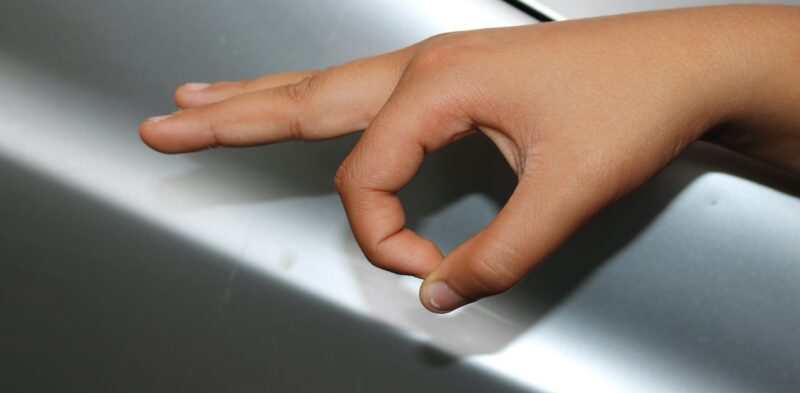
\includegraphics[width= 0.8\textwidth]{images/Chapter1/immagine.jpg} 
    \caption{Questa è un'immagine} 
    \label{fig:immagine}
\end{figure}

Questa è una citazione \cite{LabelPerLaCitazione}.

\subsubsection{Transition}

Quello che segue è un esempio di codice. E' possibile modificare il linguaggio per il synyax highlight, aggiungere parole chiave... E' tutto disponibile nella guida del pacchetto \texttt{listings}.

\lstinputlisting[language=C++]{listings/Capitolo1/code1.cpp} 

\section{Company Profile}

\lipsum[4]

\subsection{Company Type}

La tabella si indirizza sempre con l'uso di una label, ottenendo il risultato \autoref{tab:labelTabella}.

\begin{table}
    \caption{Una simpatica tabella!}\label{tab:labelTabella}
    \begin{center}
    \begin{tabular}{c|c|c|c}
        \textbf{Colonna 1} & \textbf{Colonna 2} & \textbf{Colonna 3} & \textbf{Colonna 4} \\
        \hline
            $3$      & $24$     & $24$    & $29$ \\ 
            $36$     & $31$     & $49$    & $39$ \\ 
            $32$     & $41$     & $59$    & $57$ \\ 
            $34$     & $60$     & $79$    & $74$ \\ 
            $328$    & $96$     & $194$   & $99$ \\ 
            $356$    & $117$    & $297$   & $149$ \\ 
            $312$    & $315$    & $293$   & $242$ \\ 
            $3024$   & $184$    & $253$   & $019$ \\ 
            $3048$   & $7795$   & $253$   & $077$ \\ 
            $3096$   & $7767$   & $2432$  & $0514$ \\ 
            $3192$   & $3769$   & $2435$  & $0551$ \\ 
            $36384$  & $6625$   & $3432$  & $0497$ \\ 
            $32768$  & $15469$  & $6472$  & $0471$ \\ 
            $35536$  & $15425$  & $14539$ & $10289$ \\ 
            $331072$ & $34623$  & $24941$ & $20444$ \\  
        \end{tabular}
    \end{center}
\end{table}

\appendix

\chapter{References}

\begin{enumerate}
    \item Kaz Software: \url{https://kaz.com.bd/}
    \item Our Services: \url{https://kaz.com.bd/services/}
    \item Our Culture: \url{https://kaz.com.bd/company-culture}
    \item Typescript: \url{https://www.typescriptlang.org/}
    \item ReactJS: \url{https://reactjs.org/}
    \item Redux: \url{https://redux.js.org/}
    \item Git: \url{https://git-scm.com/}
    \item Visual Studio Code: \url{https://code.visualstudio.com/}
    \item Single SPA: \url{https://single-spa.js.org/}
    \item Cypress: \url{https://www.cypress.io/}
    \item Docker: \url{https://www.docker.com/}
    \item Kubernetes: \url{https://kubernetes.io/}
    \item Prothom Shurjo: \url{https://www.facebook.com/ProthomSurjoBD}
    \item Micro-Frontends POC: \url{https://github.com/KhanShaheb34/react-microfrontends/}
\end{enumerate}


% \bibliographystyle{plain}
% \bibliography{chapters/Biblio.bib}

\end{document}
% -----------------------------------------------------------------
